\documentclass[30pt,a4paper]{article}
% Dokumenten Typ, titelseite, Schriftgröße, Seitenformat
\PassOptionsToPackage{dvipsnames}{xcolor}
% Füge neue Farben hinzu (standart 5 farben oder so)
\usepackage[utf8]{inputenc}
% Kodierung
\usepackage[T1]{fontenc}
% Umlaute
\usepackage[english]{babel}
% Eingebundene Sprachen
\usepackage{graphicx}
% Einbinden von Grafiken
\usepackage{wrapfig}
% Text um kleine Grafiken herumsetzen
\usepackage{amsmath}
\usepackage{amsfonts}
\usepackage{amssymb}
% Mathe Symbole und Commands
\usepackage{mathtools}
% Verbessert ams Packete von oben
\usepackage{nicefrac}
% Schönere Brüche
\usepackage{tikz}
\usepackage{circuitikz}
\usepackage{tikz-cd}
% Tikz Stuff
\usepackage{enumerate}
% Bessere Aufzählungen
\usepackage{cancel}
% z.B Durchstreichen von Sachen
\usepackage[hidelinks]{hyperref}
\usepackage{cleveref}
% Links und Referenzen innerhalb des Dokuments
\usepackage{tcolorbox}
% Wunderschöne Farbige Boxen mit Überschriften
\usepackage{caption}
% Erstellen von captions innerhalb einer Minipage
\usepackage[margin=1in]{geometry}
% Änderung der Gestaltung einer Seite (Überschreibt \documentclass)
\usepackage{placeins}
% Mit Hilfe von \FloatBarrier floats einschränken
\usepackage{booktabs}
% Bei Tabellen wird kann anstelle von \hline \toprule, \midrule und \bottomrule verwendet werden etc.
\usepackage{wasysym}
% Fügt eine Reihe von Symbolen wie Männlich Weiblich dazu
\usepackage{url}
% Füge Problemlos urls ein



\hbadness=99999 
% Löst ein Problem mit \hbox



\title{
	\large Advanced Physics Lab	SS19 \\[4mm]
	\textbf{\LARGE Experiment: Short half lives
	} \\[4mm]
	(conducted on: 2.-3.9.2019 with Krzysztof Bozek) \\}
% Titel des Experiments
\author{Erik Bode, Damian Lanzenstiel \\ (Group 103)}
% Autoren

\begin{document}
	
	\begin{titlepage}
	\maketitle
	\vspace{2cm}
	\begin{abstract}
	In the short half life experiment, the half life of $^{57}$Fe in the $14.4$\,keV state is measured with the delayed coincidence method. As the source, the Cobalt Isotope $^{57}$Co is used.
	\end{abstract}
	\end{titlepage}
	\newpage
	
	\tableofcontents
	\listoffigures
	\listoftables
	\newpage
	
	\section{Theory}
	\subsection{Radioactive Decays}
	Radioactive Decays are spontaneous processes in which a unstable atomic nucleus transforms into another lighter one while emitting other particles. Typical forms of radioactive decay are the alpha $\beta+$ and the $\beta-$decay.\\
	During the $\alpha-$decay a helium nucleus is emitted, reducing the atomic number by two. This form of decay is mainly found in heavy nucleus.\\ During the $\beta+$decay a proton transforms into a neutron and emits a positron as well as a electron-neutrino, reducing the atomic number by one.
	$$p\rightarrow n+e^++v_e$$
	On the other hand the $\beta-$decay is the reverse. It transforms a neutron into a proton and emits a electron and a electron-antineutrino. This decay increases the atomic number.
	$$n\rightarrow p+e^-+\bar{v}_e$$\\
	Another for the experiment important decay is the Electron Capture (EC) or $\epsilon-$decay. This one is similar to the $\beta+$decay since it also transforms a proton into a neutron. The difference being, that here the proton captures a electron to transform. The emitted particle is a electron-neutrino.
	$$p + e^- \rightarrow n + \bar{v}_e$$
	The captured electron is mostly from the K-shell while the resulting hole in the shell is filled by electrons from the L-shell. The remaining energy is either emitted through a X-ray photon or a Auger-electron. An Auger-electron is an electron that got the energy of an electron filling the vacancy left by electron in a lower state. The Auger-electron is therefore ejected. \\
	These decays are often accompanied by a $\gamma-$decays. When a decay occurs the daughter nucleus is mostly left in an exited state. It then decays into the ground state emitting $\gamma$-rays.\\
	Another Process similar to the $\gamma$-decay is the internal conversion (IC). Here the energy of a decay into a lower state is transmitted without radiation. That means no real photon is created to transport the energy. The energy is directly absorbed by another electron from the shell and ejected. The hole is filled similar to the one of EC by X-ray or Auger-electrons. 
	\subsection{Interaction between Matter and $\gamma-$Photons}	
 	When $\gamma-$photons and matter interact this happens mostly in 3 different ways depending on the atomic number of the atoms in the matter, as well as the Energy $E_\gamma$ of the photons.
 	\begin{enumerate}
 		\item Photoelectric effect:\\
 		The photoelectric effect happens when a photon is absorbed by an electron inside the matter. The energy carried by the photon is turned into kinetic energy and frees the electron. The vacancy is filled by electrons from higher shells and the energy is emitted by an Auger-electron or X-ray.\\
 		This effect appears mostly by $E_\gamma<200$\,keV and an atomic number around 50.
 		\item Compton scattering:\\
 		Unlike the photoelectric effect the photons are not absorbed by the electrons in the matter. They give up a part of their energy and scatter at the electron.\\
 		The Compton scattering happens by Energies in the range of $200$\,keV$<E_\gamma<5$\,MeV and a atomic number similar to the photoelectric effect.
 		\item Pair Production:\\
 		Pair production is an effect that appears by an energy $E_\gamma$ over the critical one of $1.022$\,MeV. When a $\gamma$-quantum gets into the electromagnetic field of a nucleus or electron it can be converted into an electron positron pair. 
 		$$\gamma \rightarrow e^- + e^+$$
 		To create this pair the energy of $1.022$\,MeV is needed this is also the reason the pair production can't happen if the photon has less energy. The remaining energy is given to the nucleus. The positron annihilates with an electron shortly after it's creation into two $\gamma$-rays with each half $0.511$\,MeV.
 	\end{enumerate}
 	\subsection{Energy Spectrum}
 	In the energy spectrum are a few areas of interest. \\
 	First of all their are the Photo-peaks. These are peaks which come into being when a photon gives its whole energy to the detector. This will happen during a photoelectric effect if the emitted x-Ray or auger electron also gets absorbed.\\
 	Another region of interest (ROI) could be the Escape-peak. Here the x-Ray emitted by an exited state dropping to back to the ground state leaves the detector without interaction. That means the Escape-peak will be shifted by the amount of energy that left the detector.\\
 	The next point is the Compton edge and spectrum. If the emitted photon only interacts with the detector only by Compton scattering, and leaves the detector only a part of the energy will be deposed. This energy will form the Compton-spectrum. For a scattering angle of $180$ the maximum amount of energy will be absorbed. This energy symbols the abrupt end of this spectrum and is called the Compton-edge.\\
 	Last but not least there is the Backscatter-peak happens through photons that get scattered at material outside of the detector and find their way back in where they get absorbed. That way they lose some energy depending on the material. This is way the peak is shifted by this amount from the position of the Photo-peak. 
 	\subsection{Methodology}
 	\ \\ 
 	\begin{wrapfigure}{l}{8cm}
 		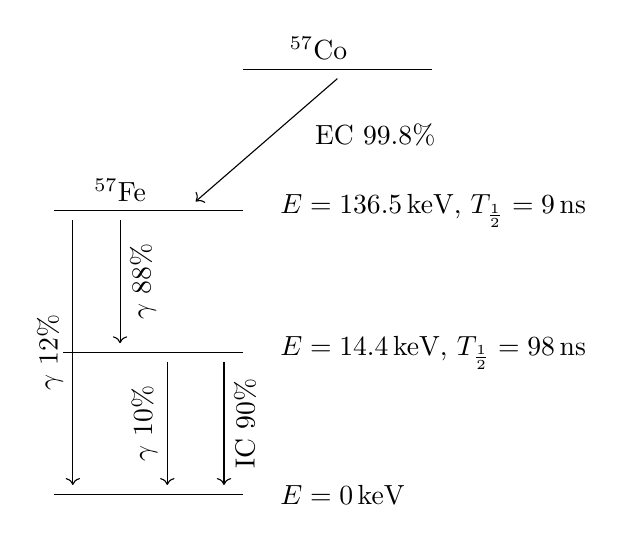
\begin{tikzpicture}[scale=1.2]
 		\draw (1,1.5) -- (1.8,1.5) node[above]{$^{57}$Co} -- (3,1.5);
 		\draw[->] (2,1.4) -- (0.5,0.1);
 		\node at (2.4,0.8) {EC $99.8\%$};
 		\draw (-1,0) -- (-0.3,0) node[above]{$^{57}$Fe} -- (1,0) node[right]{\quad$E=136.5$\,keV, $T_\frac{1}{2}=9$\,ns};
 		\draw (-0.9,-1.5) -- (1,-1.5) node[right]{\quad $E=14.4$\,keV, $T_\frac{1}{2}=98$\,ns};
 		\draw (-1,-3) -- (1,-3) node[right]{\quad$E=0$\,keV};
	 	\draw[->] (-0.8,-0.1) -- node[rotate=90,above]{$\gamma$ 	$12\%$} (-0.8,-2.9);
 		\draw[->] (0.2,-1.6) -- node[rotate=90,above]{$\gamma$ $10\%$}(0.2,-2.9);
 		\draw[->] (-0.3,-0.1) -- node[rotate=90,below]{$\gamma$ $88\%$} (-0.3,-1.4);
 		\draw[->] (0.8,-1.6) -- node[rotate=90,below]{IC $90\%$} (0.8,-2.9);
 		\end{tikzpicture}
 		\caption{\small Decay scheme for the cobalt isotope $^{57}$Co into $^{57}$Fe used into the experiment to measure the half-life of the $14.4$\,keV state of the Iron isotope.}
 		\label{CoDecay}
 	\end{wrapfigure}
 	\ \\ 
 	To measure the half-life of $^{57}$Fe we use the decay of the $^{57}$Co Isotope (see figure \ref{CoDecay}) $^{57}$Co decays by EC into an exited state of $^{57}$Fe. At this point it can either decay directly to the ground state emitting a $\gamma$-photon.\\
 	The more likely case with $88\%$ is, that it first goes to the wanted state of $14.4$\,keV by emitting a $\gamma-$ray. From this state it again has two options. With a $90\%$ probability we have an IC which we can't detect but there is also a $10\%$ chance that a $\gamma-$decay takes place.\\
 	\ \\
 	To measure the half-life it makes sense to use the method of delayed coincidence. For this kind of measurement we need to measure the time $\Delta t$ it takes for the $14.4$\,keV state to decay. The $\gamma$-photons connected to this state can be used to track the creation and the decay of the measured state and with that our time $\Delta  t$. This time is of interest since like the radioactive decay which is a stochastic process, it follows the equation \ref{eq1}.
 	\begin{equation}
 		N(t)=N(0) e^{\frac{t}{\tau}}=N(0) *2^{\nicefrac{t}{T_\frac{1}{2}}}
 		\label{eq1}
 	\end{equation}
 	\begin{enumerate}
 		\item[•] $N(t)$: Number of existing nucleus at a given time.
 		\item[•] $N(0)$: Number of nucleus at the time zero.
 		\item[•] $\tau$: Mean life time of the decaying quantity.
 		\item[•] $T_\frac{1}{2}$: Half-life of the decaying quantity.
 	\end{enumerate}
	With that the amount of measured decays at certain times $\Delta t$ the half-life can be calculated. A problem that appears for the used decay is the rarity of the $\gamma$-ray with $14.4$\.keV. This one has only a $10\%$ chance of appearing and stopping our measurement. That would lead to a long dead time in which no new measurement can be taken. The problem is easily solved by using the rarer signal as the start of the measurement and stopping it with the $122$\,keV photon. Since there are also random coincidences which will distort the measurement a background measurement has to be made. This one can be subtracted from the real measurement.
 	
 	\subsection{$\gamma$-Ray Detection}
 	To detect the $\gamma$-rays two scintillators which react to the $\gamma$-photons exhibiting scintillation will be used. This again can be detected by a photomultiplier tube (PMT) and converts them into an electric pulse.\\
 	As scintillators organic and inorganic ones can be used. The main difference being the decay time of the emission centers and the luminous efficiency. If the half-life is bigger than $10^{-9}$\,s inorganic Naj(Tl)-scintillators are the choice since they have the higher luminous efficiency. For shorter times organic ones have to be used because of the shorter decay time.\\ For this experiment inorganic ones can still be utilized. The light from emitted can by light transmission bars to the PMTs. That way the loss will be minimized. \\ The PMT is used to generate an electric signal by using the photoelectric effect. The pulse is increased by using increasing the velocity of the electrons freed by the photons and using them to free even more electrons at the dynode. This process will be repeated till a useful signal is produced.
 	\section{Experimental Setup}
 	In the first part of the experiment the energy spectrum of $^57$Co and $^241$Am are measured. For this the setup in figure \ref{setup_ES} is used.
 	\begin{figure}
 		
\includegraphics{Bilder/Circuit_ES}
 	\end{figure}
 
 	
 	
\end{document}